% theKATRINexperiment.tex
%

    \chapter{KATRIN experiment}
    \label{ch:The KATRIN experiment}
    The KATRIN experiment is urrently being assembled at the Karlsruhe Institute of Technology to determine the effective mass of the electron anti-neutrino with a sensitivity of \SI{200}{\milli\electronvolt}/\SI{}{\square c} at \SI{90}{\percent} C.L., excelling the predecessor  experiments at Mainz and Troisk by a factor of \SI{10}{}. Major challenges of the project are the required ultra high vacuum, the exact knowledge of all magnetic and electric fields as well as external influences on those, the required high luminosity of the tritium source and the classification and reduction of background sources. This chapter will give an overview of the measurement principle of KATRIN (section \ref{ch:The KATRIN experiment:sec:Measurement Principle}) and the experimental setup (section \ref{ch:The KATRIN experiment:sec:Experimental setup}).
    
      \section{Measurement principle}
      \label{ch:The KATRIN experiment:sec:Measurement Principle}
      The general idea of the KATRIN experiment is a high-precision measurement of the energy of electrons from tritium decay 
      \begin{equation}
      	\ce{^3_1T -> ^3_1H^+ + e^- + \bar{\nu}_e}.
      \end{equation}
      and a comparison to the spectral shape as obtained for a massless neutrino \cite{Otten:2008zz}.
      As the decay energy is distributed between the rest mass of the decay products and the kinetic energies the neutrino and the electron respectively, the decay electrons show a continuous spectrum. The difference between the spectral shape calculated with Standard Model presumptions and the measured shape are used to determine the neutrino mass. As all three mass eigenstates contribute to the electron neutrino mass in any scenario (see figure \ref{ch:Introduction:sec:neutrino Oscillations}), the difference will be a superposition of these. The kinks occurring for each individual mass eigenstate can not be resolved with the KATRIN spectrometer as the energy resolution is larger than the mass differences. As all three flavors contribute to the electron neutrino mass, what will be measured is the incoherent sum will be measured as described in section \ref{ch:Introduction:sec:Neutrinos in the Standard Model}.
      
      \begin{figure}
	\centering
      	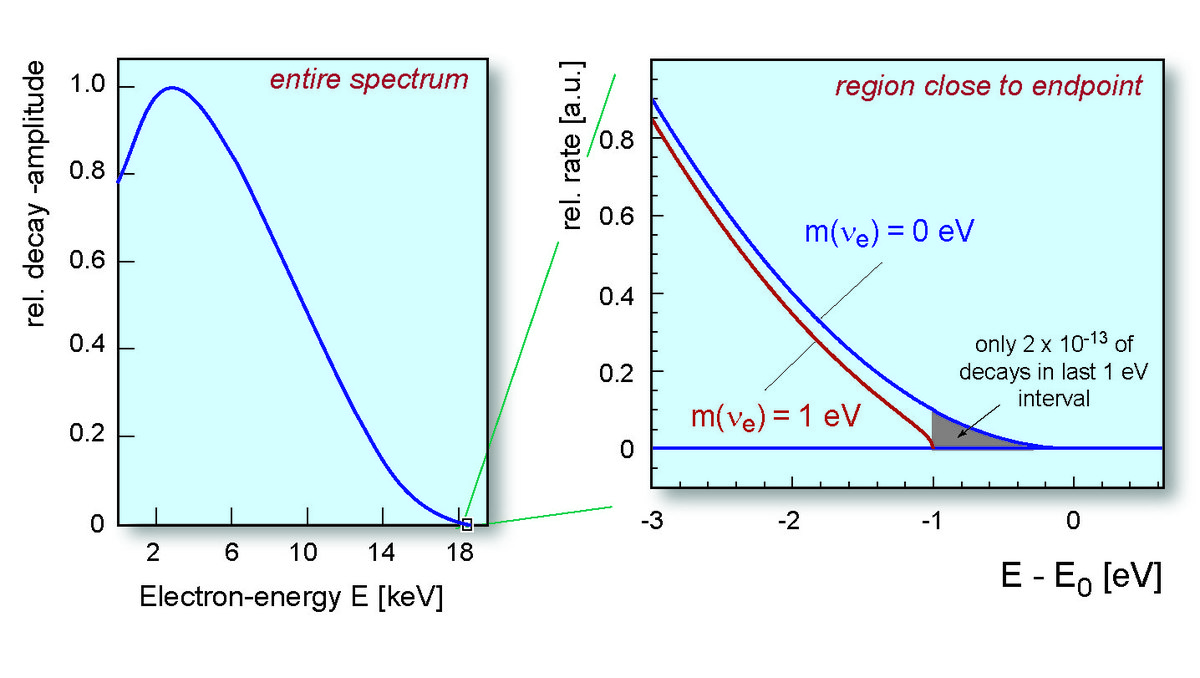
\includegraphics[width = 0.9 \textwidth]{graphics/katrinExperiment/electronSpectrum.jpg}
      	\caption[Schematic Tritium Energy Spectrum]{Schematic energy spectrum for electrons from tritium beta decay. On the left, the entire spectrum peaking around \SI{5}{\kilo\electronvolt} - can be seen. On the right, a zoom-in to the endpoint region shows the calculated spectra for a massless neutrino and a massive neutrino with m=\SI{1}{\electronvolt} neutrino. As described in the graph, rates in this region are extremely low and sophisticated analysis tools have to be applied.}
      	\label{fig:katrinExperiment:tritiumSpectrum}
      \end{figure}
      One of the major challenges is the exact determination of the electron energy with an energy resolution of \SI{0.93}{\electronvolt}, required to achieve the design sensitivity \cite{KATRINWolf}. While each component of the experimental setup by itself already exhausts the current technological limits, they also have to work in combination with each other. In the context of this thesis, it is important to notice that stringent requirements concerning the background contribution of each component have to be met to achieve the design goal.
       \subsection{MAC-E Filter}
                   \begin{figure}
	\centering
      	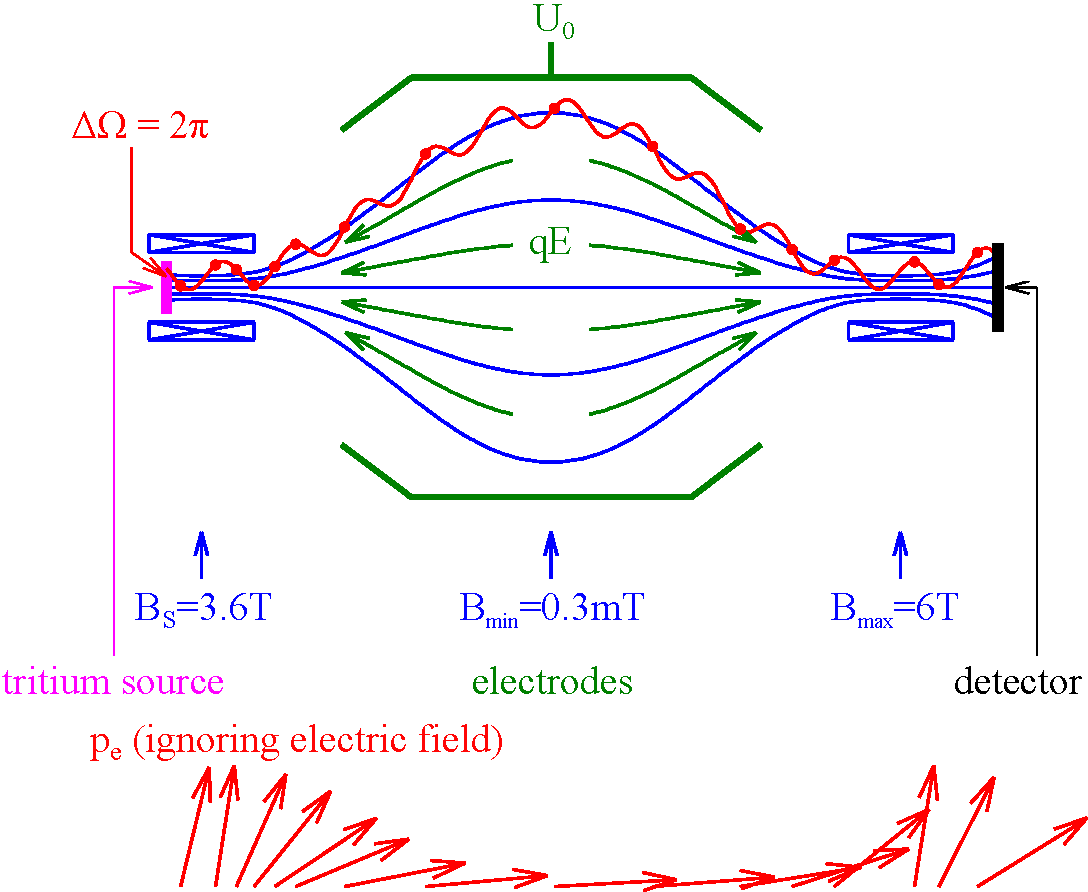
\includegraphics[width = 0.8 \textwidth]{graphics/katrinExperiment/macEFilter.pdf}
      	\caption[MAC E Filter]{Principle of a MAC E filter. In the upper part, magnetic field lines are plotted in blue together with the field values at the source (\SI{3.6}{\tesla}) and inside the pinch solenoid (\SI{6}{\tesla}). The accepted solid angle and an exemplary particle path are shown in red. The analyzing plane is defined by the area of minimum magnetic fields $B_{min}$. Below, the momentum of an electron with a large starting angle with respect to the magnetic field lines is shown. It tips over as the field weakens. Meanwhile (not shown in this graph), the vessel voltage $U_0$ analyses the energy parallel to the electric field allowing only electrons with large enough energies to pass on to the detector \cite{macEFilter}.}
      	\label{fig:katrinExperiment:macEFilter}
      \end{figure}
      \label{ch:The KATRIN experiment:sec:MAC-E}
		To measure the energy of electrically charged decay electrons at high precision, an electrostatic filter is best suited. As the electrons are emitted isotropically, they will have momentum components both parallel and perpendicular to the source-detector axis (defined as the z-axis). To determine the total electron energy, the momentum direction needs to be well defined. In case of an electrostatic filter, only the parallel component can be analyzed.
		At the same time, a high luminosity is a major requirement for good statistics for the KATRIN experiment.
		To satisfy all these requirements, several techniques are combined in the MAC-E filter, the magnetic adiabatic collimation with electrostatic filter \cite{katrinPrinciple}.\\\\
		{\bf Magnetic} field lines connect the source and the detector. Electrons from tritium decays are guided from the source to the detector, thereby performing cyclotron orbits around the magnetic field lines. Consequently, a maximal solid acceptance angle of 2$\pi$ can be achieved, resulting in a high luminosity at the detector.\\\\
		{\bf Adiabatic} electron motion in the magnetic field is achieved if the magnetic field change is small within each cyclotron orbit. In this case, the magnetic momentum $\mu$, which is correlated to $E_\bot$, the energy perpendicular to the magnetic field $B$, remains constant
		\begin{equation}
			\mu = \frac{E_{\bot}}{B} = const \propto \frac{p^2_\bot}{B}.
			\label{eq:magMomentum}
		\end{equation}
		{\bf Collimation} in a MAC-E filter is based on the above adiabacity. The magnetic field strength drops by four orders of magnitude from $B_{max}$ at the superconducting solenoids to $B_{min}$ in the analyzing plane (see figure \ref{fig:katrinExperiment:macEFilter}). Following equation \ref{eq:magMomentum}, this means that the energy perpendicular to the magnetic field has to drop accordingly for $\mu$ to remain constant. This leads to a parallelization of momentum vector and B-field direction. \\\\
		{\bf Electrostatic filtering} occurs exactly at the point of minimal energies $E_\bot$ in the analyzing plane. Here, the momentum vector is aligned mostly parallel to the magnetic field $E_{||}$, which determines the parallel energy component. Setting the electrostatic filter to a fixed voltage $U$ now reflects electrons with $E_{||} < U\cdot e$.\\
		As electrons are emitted isotropically in the source, they exhibit an energy $E_\bot \neq 0$. Therefore, electrons in the analyzing plane have remaining energy $E_\bot$, which limits the filter resolution 
		\begin{equation}
			\mu_{low} = \frac{E_{\bot_{min}}}{B_{min}} = \frac{E_{\bot_{max}}}{B_{max}} = \mu_{high} = \mu,
		\end{equation}

		the relative sharpness is given by the maximum transversal energy $E_{\bot_{max}}$ that is still accepted by the filter:
		\begin{equation}
		\Delta E = E_{\bot_{max}} = E_{0}\frac{B_{min}}{B_{max}}
% 			\frac{\Delta E}{E} = \frac{B_{min}}{B_{max}}.
		\end{equation}
		
		Only in the unachievable case of $B = 0$ in the analysing plane, the momentum would be exactly parallel to the field and the resolution would not be limited. The main spectrometer reaches a resolution of \SI{0.93}{\electronvolt} (see section \ref{ch:The KATRIN experiment:sec:Experimental setup:subsec:MainSpec} for more details).
		After passing the analysing plane, the electrons are reaccelerated by the electric field and guided and focused onto a detector by the magnetic field.
		To additionally dismiss electrons with large starting angles, the source field strengths are chosen to be smaller than the maximum field strength inside the pinch solenoid. This measure ensures that electrons with long paths that are consequently more likely to scatter off tritium molecules in the source will not be analyzed using the effect of magnetic mirroring \cite{magneticMirror}.
		With the chosen settings, this results in an angular acceptance of \SI{50.77}{\degree}. 
% 		\begin{equation}
% 			\mu_{\mathrm{0}} = \mu_{\mathrm{low}} ~ \longrightarrow ~ \frac{E_{\bot_0}}{B_0} = \frac{E_{\bot_{low}}}{B_{low}} 
% 		\end{equation}
%       To further filter out electrons with high starting angle, the source is set to lower fields than the maximum $B_{max}$.
%       As with larger angles come longer paths, this reduces the probability of electrons taking part in scattering processes inside the source section being detected.
%       \begin{equation}
%       	\theta_{s~max}= \arcsin{\sqrt{\frac{B_s}{B_{max}}}}
%       \end{equation}
%       

      

      \section{Experimental Setup}
      \label{ch:The KATRIN experiment:sec:Experimental setup}
      The KATRIN experiment consists of different sections all fulfilling their own important purpose in the whole setup. Located at one end is the windowless gaseous tritium source ``WGTS''. Here, tritium decays isotropically, thereby emitting electrons. These are guided magnetically through the differential and cryogenic pumping sections, ``DPS'' and ``CPS'', removing hydrogen ions and other residual gases in the process. At the same time, at the other end of the WGTS, the rear section scans the activity of the source. For the electrons on their way to the detector, the path continues through the two spectrometers acting as a energetic high pass filters to the focal plane detector, ``FPD'', registering them.\\
      During the whole procedure, the electrons from the decay may not undergo energy changes as the exact knowledge of their kinetic energy is essential to the experiment. Consequently the guiding needs to be adiabatic, which is guaranteed by spatially slowly changing and temporally constant magnetic fields.\\
      Figure \ref{fig:beamLine} shows a schematic overview of the whole experimental setup. It follows a more detailed description of the individual components.
      
      \begin{figure}
			
      		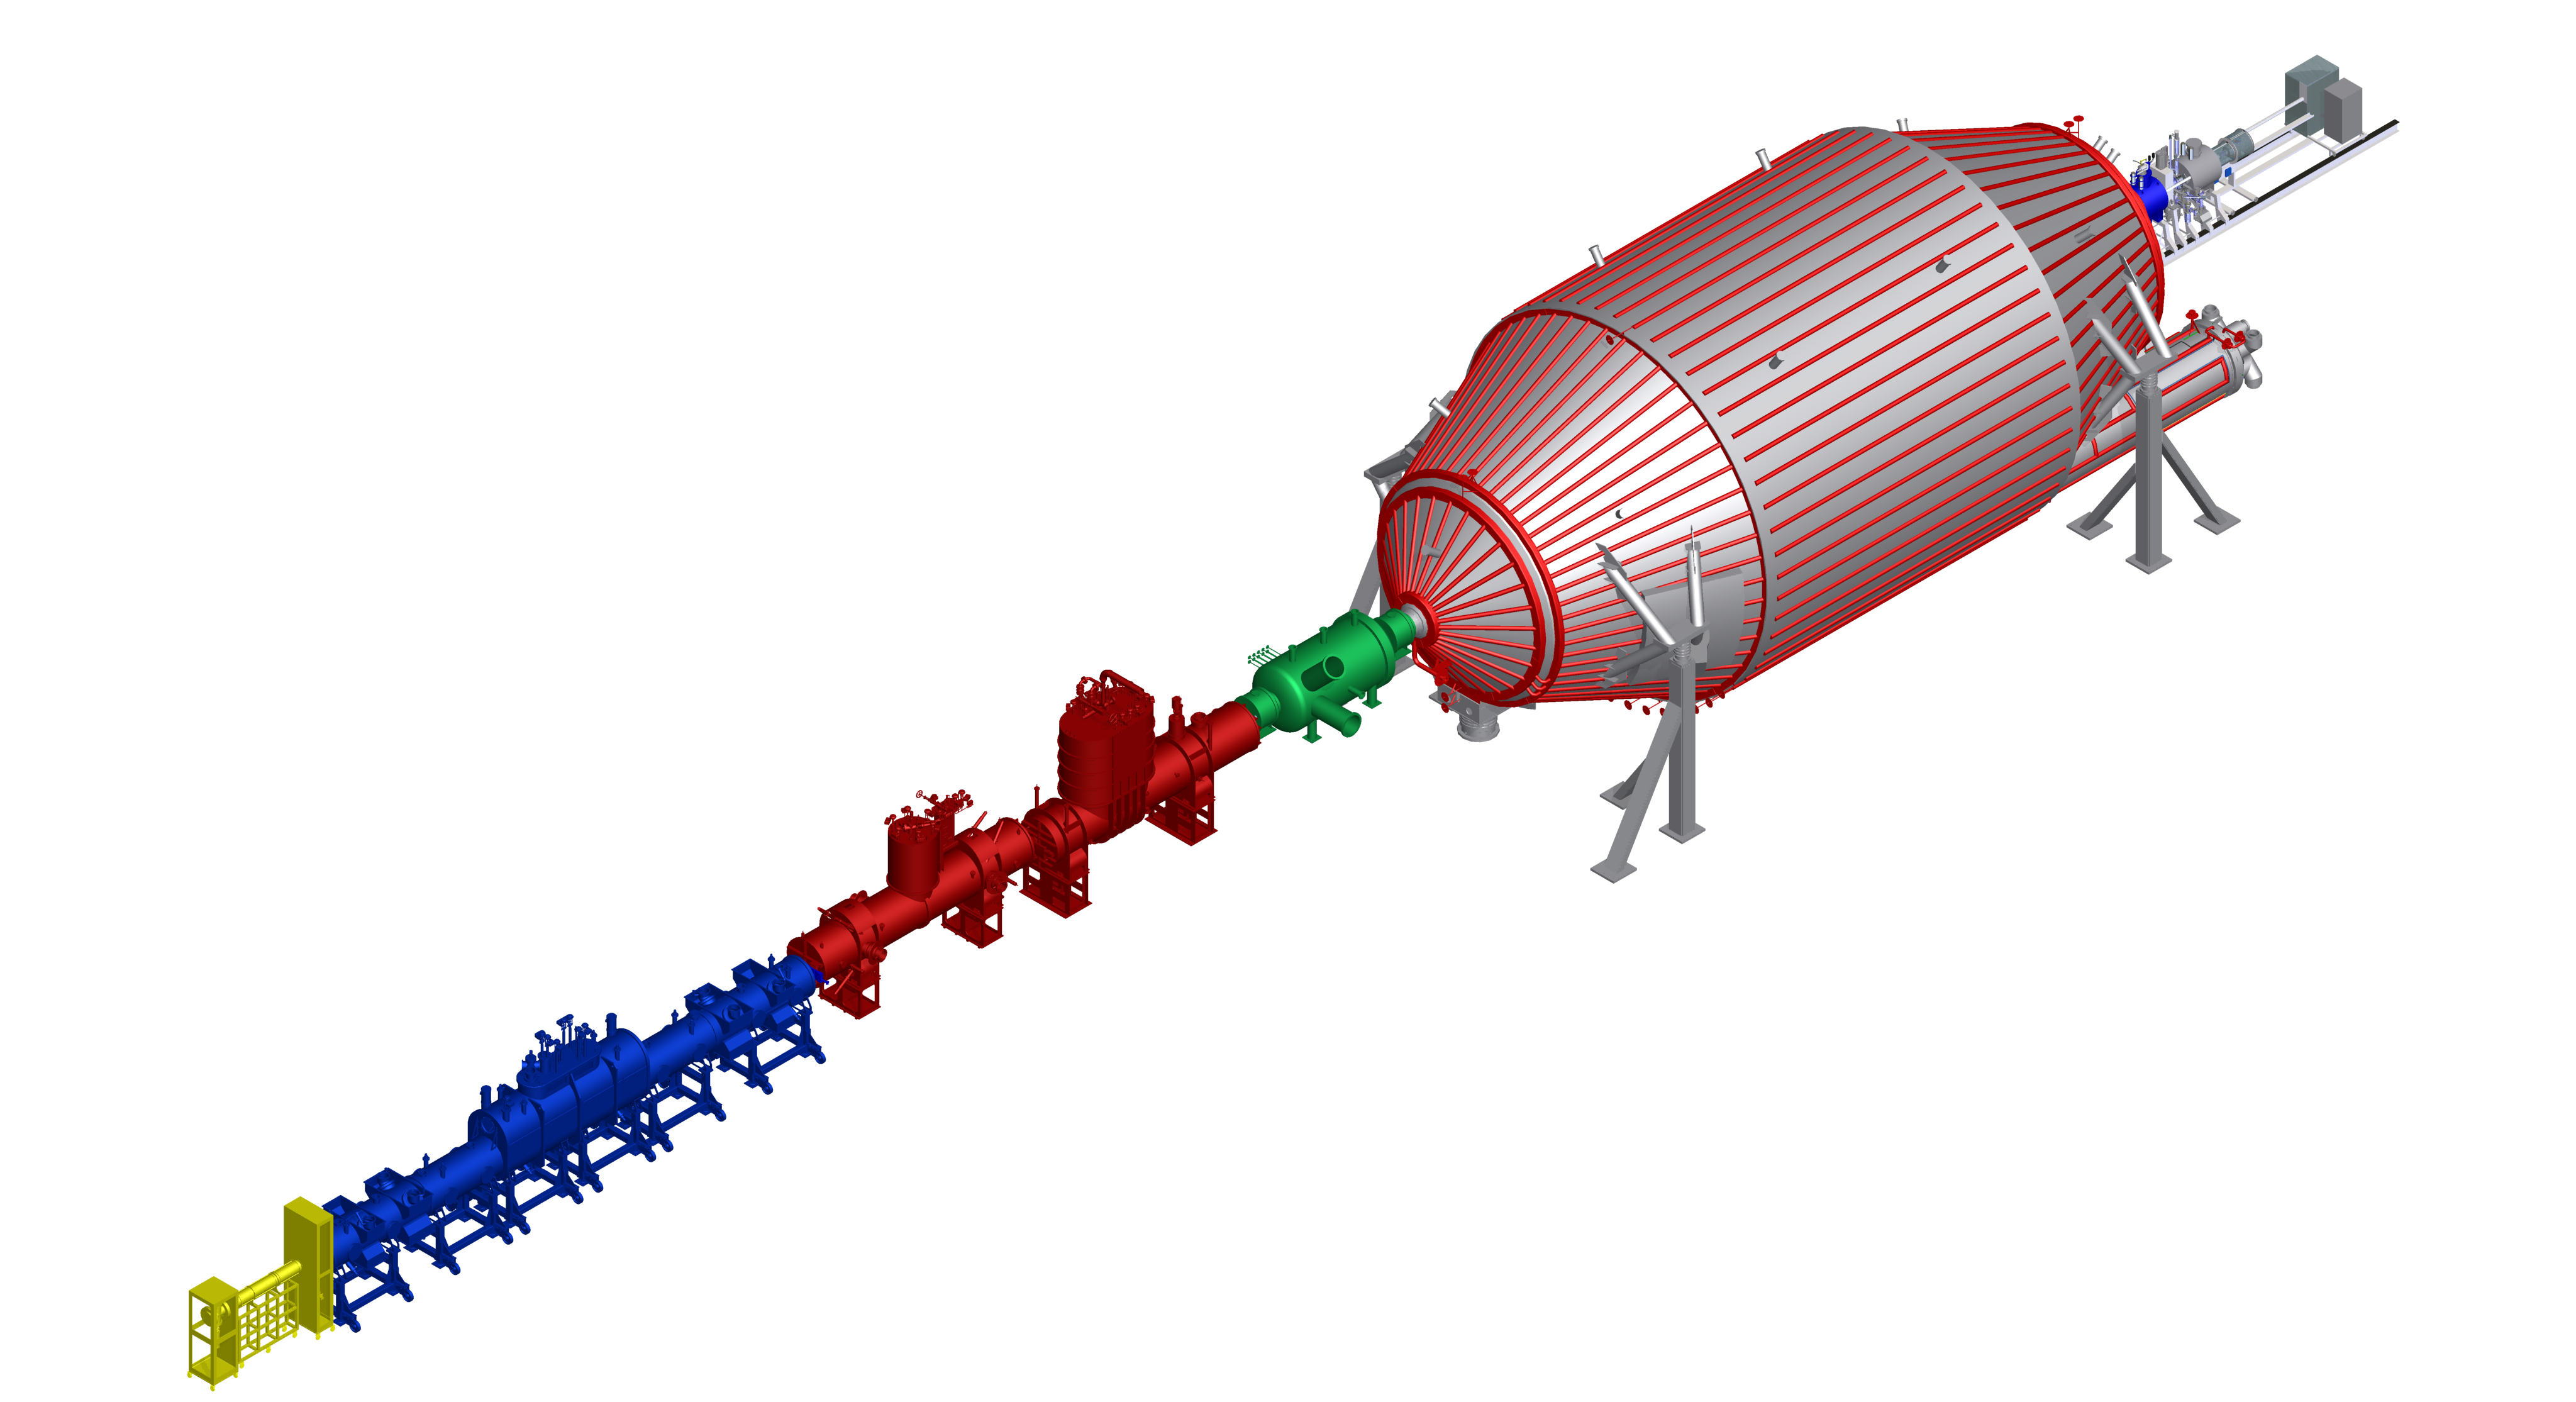
\includegraphics[width = \textwidth]{graphics/katrinExperiment/beamLineHD.jpg}

      	\caption[KATRIN Beam Line]{The beam line of the KATRIN experiment with the different stages: Rear section (yellow) and WGTS (blue) on the very left, followed by the transport section (red) consisting of DPS and CPS. Energy analysis in pre- (green) and main spectrometer (grey-red) of the spectrometer section and electron detection at the detector section (grey-blue).}
      	\label{fig:beamLine}
      \end{figure}

      
      \subsection{WGTS and Rear Section}
      \label{ch:The KATRIN experiment:sec:Experimental setup:subsec:sourceSide}
      A gaseous tritium source, shown in figure \ref{fig:sourceSide}, is utilized to generate tritium decay electrons. Advantages of the employed principle are the absence of solid state effects and a high luminosity \cite{letterOfIntent}. In a solid, like tritium films, most decay electrons from inside the solid would interact with the solid itself, which leads to energy losses imitating a non-zero neutrino mass. Additionally, not only the surface facing the detector emits electrons at the required spectrum, but the electrons from the whole volume covered by the magnetic flux tube hitting the detector can be analyzed. Furthermore, the emission of this kind of source is very homogeneous. However, new challenges arise when using gas instead of solids.
      \begin{itemize}
		\item The source temperature needs to be very stable with a maximum deviation of \SI{\pm0.03}{\kelvin} at \SI{30}{\kelvin}, to guarantee a rate stability of \SI{\pm0.1}{\percent} for the decay electrons \cite{temperatureWGTS}.
      	\item The spectrometers further downstream require an ultra high vacuum - \SI{e-11}{\milli\bar} or better in case of the main spectrometer. With a tritium pressure is in the order of \SI{e-3}{\milli\bar} inside the windowless source the pressure must be reduced to a partial pressure of $10^-19$ mbar inside the main spectrometer without any physical barrier.
      	\item The contribution of the individual hydrogen isotopologues of the gas has to be known precisely. For this purpose a laser-raman-system has been developed \cite{calibrationRaman}.
      	\item All devices used in contact with tritium have to undergo excessive testing in tritium environment to guarantee failure safety under the harsh conditions.
      \end{itemize}
      
     \begin{figure}
     \centering
		\begin{minipage}{0.6\textwidth}
				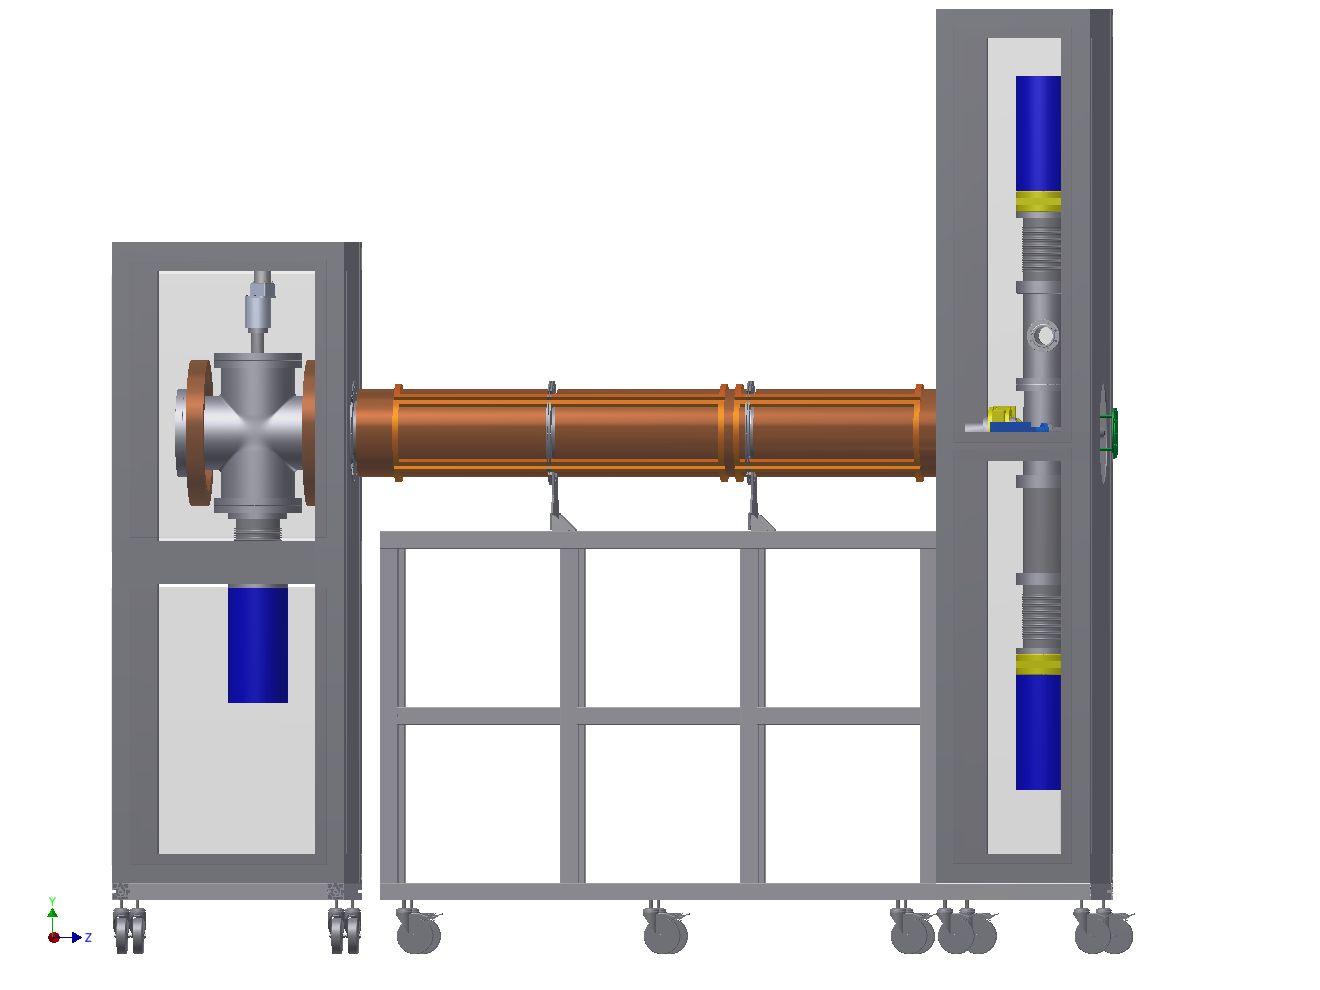
\includegraphics[width = 1.0\textwidth]{graphics/katrinExperiment/rearSectionFull1.png}
		\end{minipage}
		\begin{minipage}{\textwidth}
			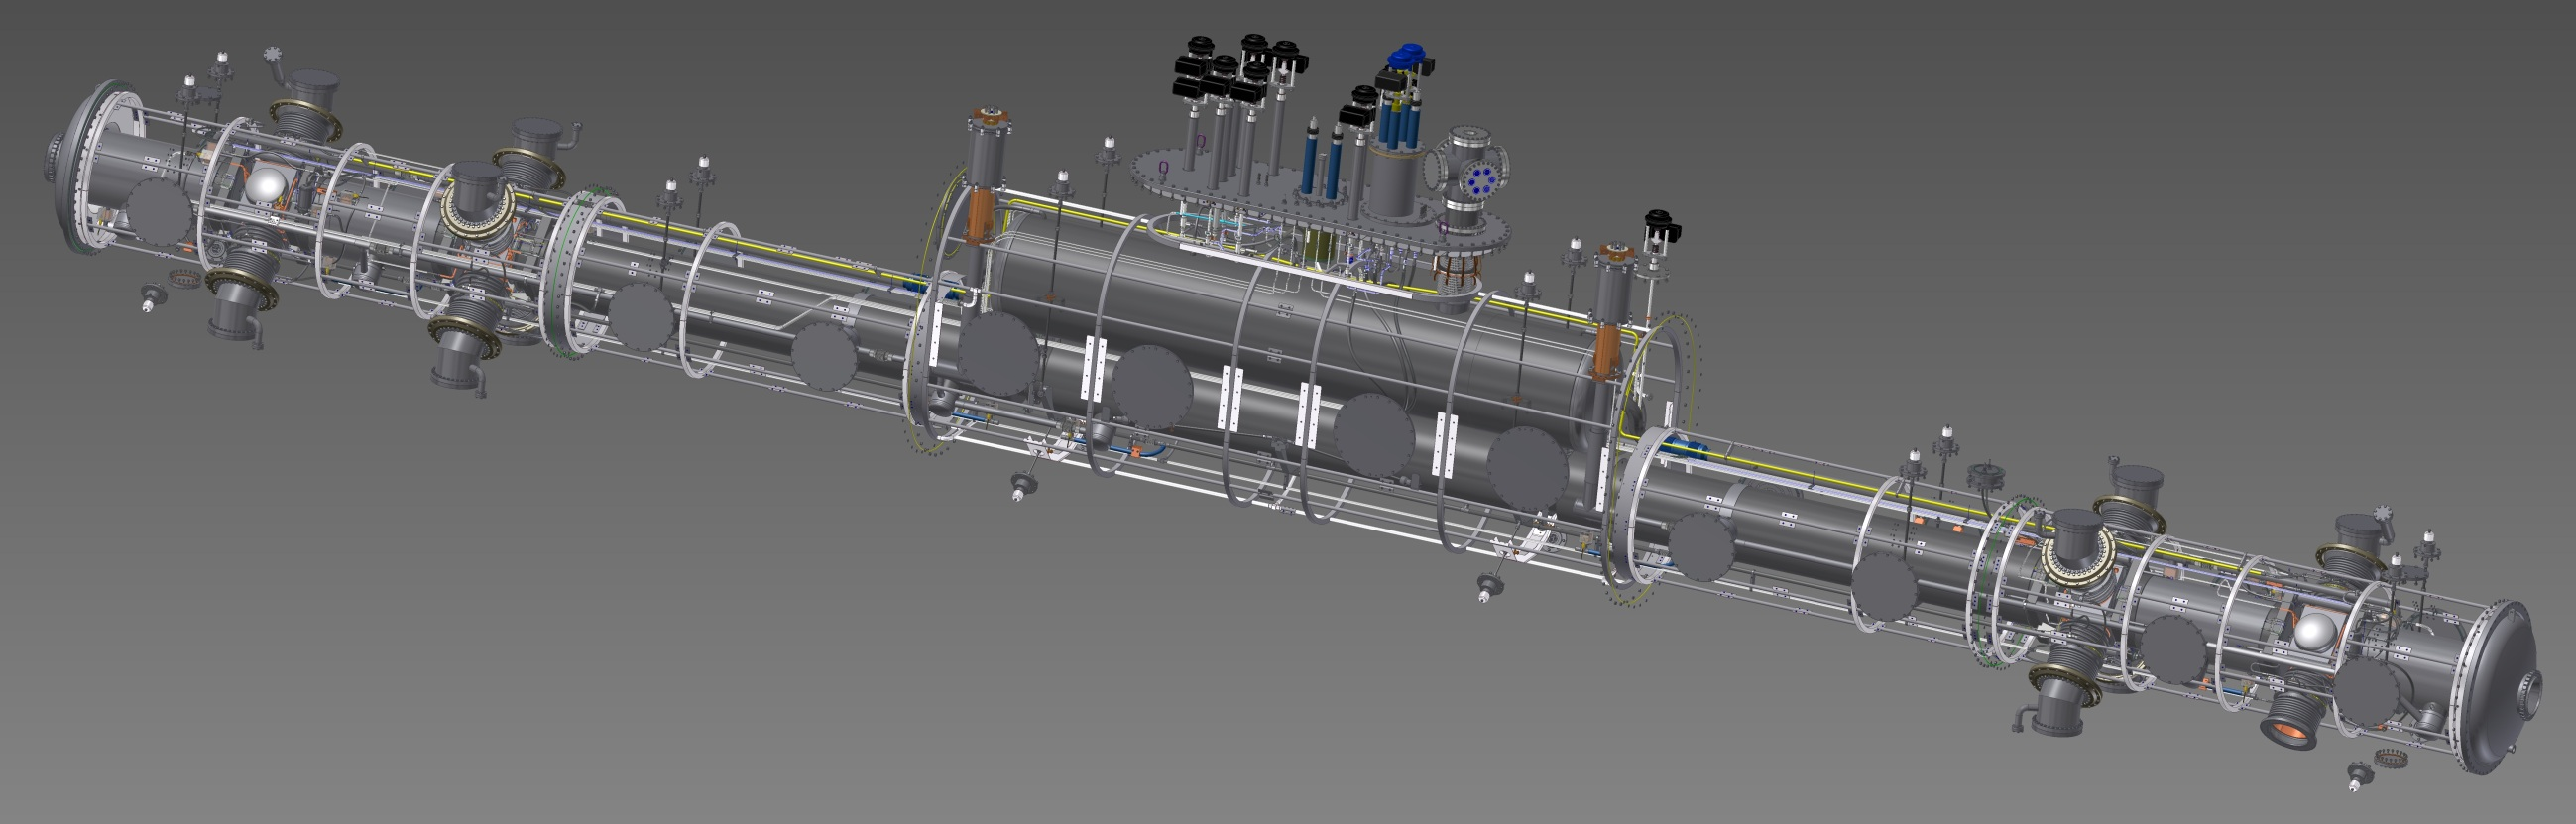
\includegraphics[width = 1.0\textwidth]{graphics/katrinExperiment/WGTS.jpg}
		\end{minipage}
		\caption[Rear Section and WGTS]{Top: the rear section. In the model, there are two large attachments visible perpendicular to the beam direction. The right one is the e-gun for calibration purposes.The left one is the rear wall, which is responsible for monitoring of the source activity. Also visible are the gray second containment boxes required for redundancy in radiation security. Bottom: a model of the WGTS. The large number of pumping ports is clearly visible on the left and right end. Tritium is injected in the middle of the central tube from where it diffuses to both ends of the WGTS. Images from \cite{rearSection} and \cite{WGTSDrexlin}.}
		\label{fig:sourceSide}
      \end{figure}
      
      
      \subsection{Transport Section}      
      Figure 2.5 shows the two sub-systems of the transport section, which are responsible for a reduction of the tritium flow by 12 orders of magnitude\footnote{A suppression by an additional 2 orders of magnitude is achieved by active pumping at the front end of the WGTS.}.
      In the differential pumping section (DPS), pressure is actively reduced by five orders of magnitude with the use of turbo molecular pumps. These as well need to be tested thoroughly to withstand the constant radiation by tritium decays \cite{tritiumTests} and the operation in strong magnetic fields. The tritium gas is then processed to be reused in the tritium cycle. Further downstream, the cryogenic pumping section (CPS) uses an ultra-cold inner surface of the tilted beam tube to freeze residual gas, while guiding the signal electrons around the chicanes by strong magnetic fields. 
      \begin{figure}
		\begin{minipage}{0.49\textwidth}
				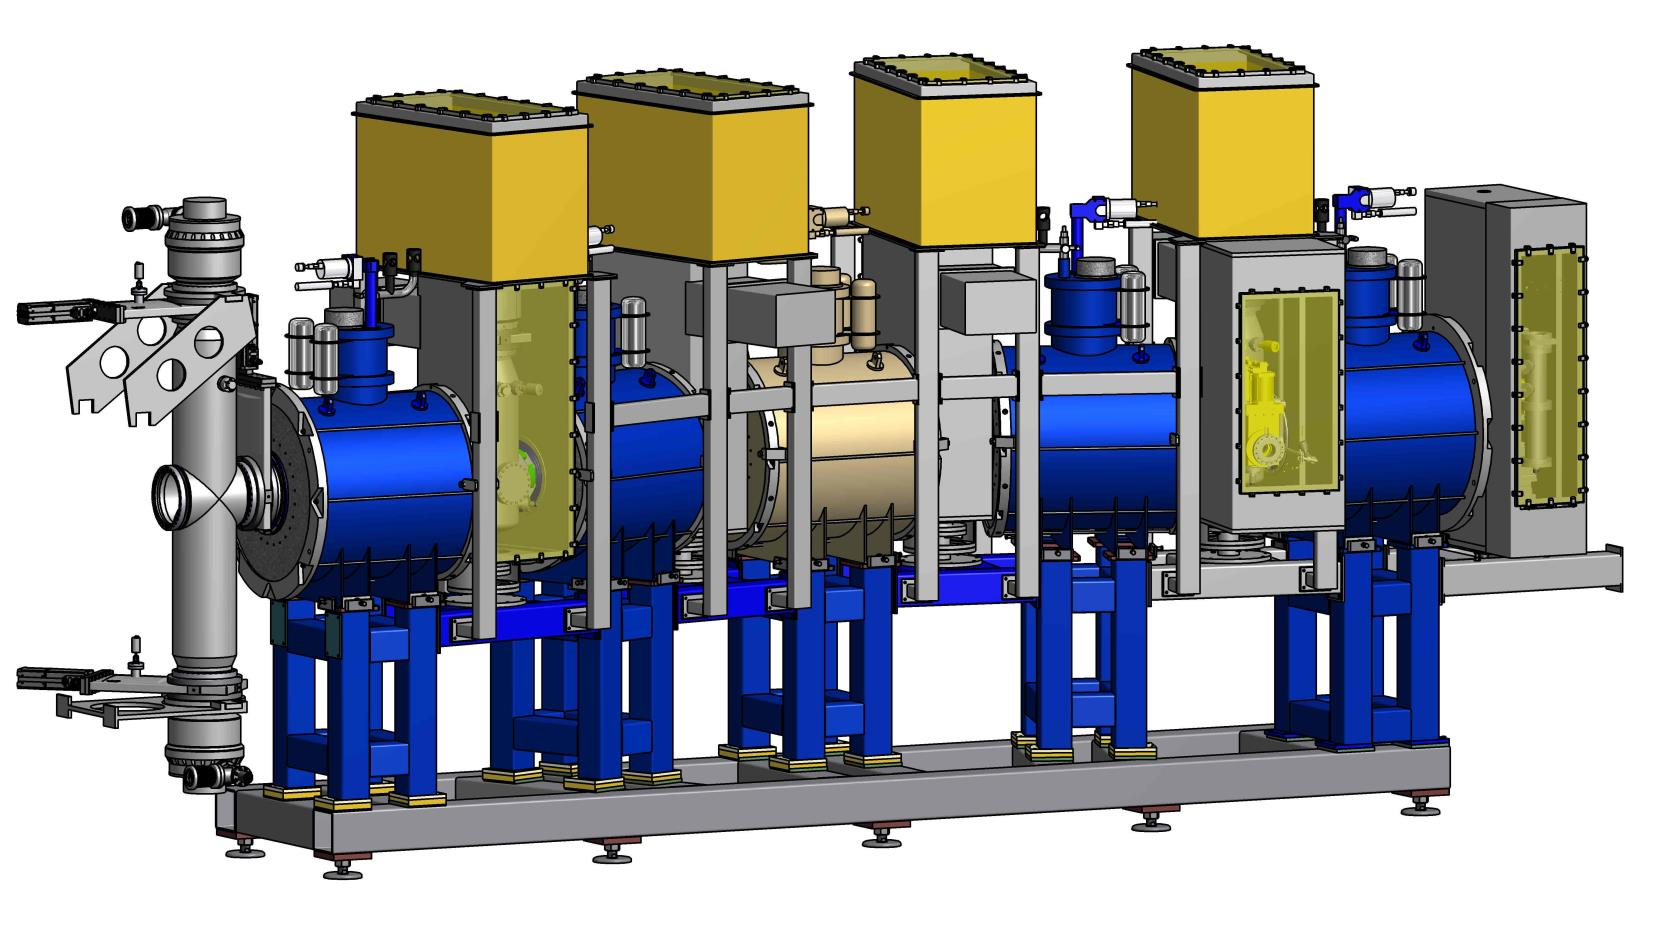
\includegraphics[width = 1.0\textwidth]{graphics/katrinExperiment/DPS.jpg}
		\end{minipage}
		\begin{minipage}{0.49\textwidth}
			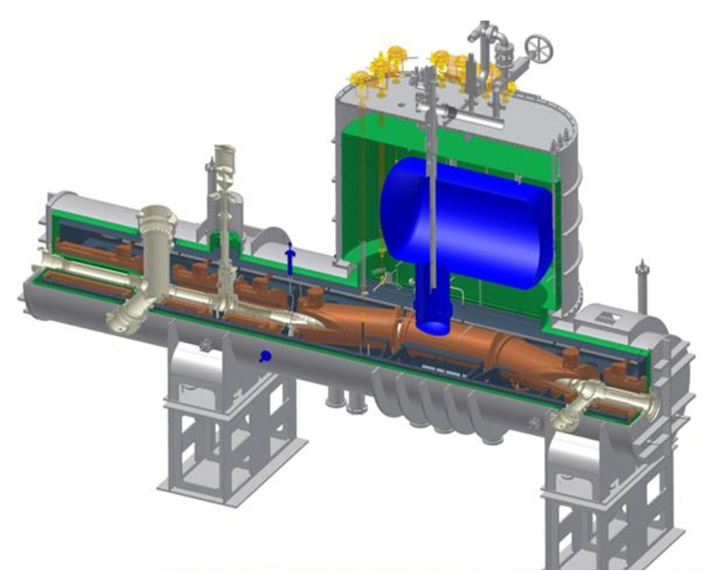
\includegraphics[width = 1.0\textwidth]{graphics/katrinExperiment/CPS.jpg}
		\end{minipage}
		\caption[DPS and CPS]{The sub-systems of the transport section. Left: the DPS with four large pumping ports along the beam line between the superconducting magnets. All the ports are isolated against the surroundings (yellow boxes) to protect against potential radiation leaks \cite{DPS}. Right: the CPS with its coolable wall structure to capture the remaining tritium-molecules \cite{CPS}.}
      \end{figure}
      
      \subsection{Pre-Spectrometer}
      \label{ch:The KATRIN experiment:sec:Experimental setup:subsec:PreSpectrometer}
      The pre-spectrometer was built to reduce the electron flux to the main spectrometer by up to 7 orders of magnitude \cite{statusPSWolf}. It works according to the MAC-E filter principle from chapter \ref{ch:The KATRIN experiment:sec:MAC-E}. With a moderate, but sufficient, energy resolution of about 60 eV, its purpose is to cut off the spectrum below energies of \SI{18.4}{\kilo\electronvolt}. Electrons above that limit will pass this pre-filter and can be further analyzed in the main spectrometer. Here, it is important that the momentum is restored after analysis which requires for a symmetric setup. To shield against externally induced electrons, the pre-spectrometer has a single layer of wires as a inner electrode. It can be set to negative voltages in comparison to the pre-spectrometer hull which then reflects electrons with energies up to $Ue$.
      
      \subsection{Main Spectrometer}
      \label{ch:The KATRIN experiment:sec:Experimental setup:subsec:MainSpec}
      The largest component in the experimental setup is the main spectrometer. With a diameter of \SI{10}{\meter} and a length of over \SI{23}{\meter}, its total volume amounts to about \SI{1400}{\cubic\meter} that need to be evacuated to extremely high vacuum of < \SI{e-11}{\milli\bar}. The main spectrometer, as the pre spectrometer, makes use of the MAC-E filtering technique described in section \ref{ch:The KATRIN experiment:sec:MAC-E}. To do so, it features a uniquely designed double-layer inner wire electrode and a sophisticated high voltage system \cite{mainSpecElectrodeDesign}. A precision voltage divider was constructed to be able to read out the high voltage applied to the vessel with the highest precision voltmeters, which operate in the range of \SI{10}{\volt} \cite{highVoltageDivider}. Additionally, the voltage is fed to the monitor spectrometer, detailed in section \ref{ch:TheKATRINexperiment:sec:experimentalSetup:subsec:monSpec} to monitor its long term stability.
      
      ne of the major background sources are secondary electrons emitted from the spectrometer surface. The magnetic field in the main spectrometer acts as an intrinsic shield against this background component. However, due to imperfections in the axial symmetry of the magnetic field, some electrons can penetrate the sensitive flux tube volume, increasing the background beyond the required value. The vessel is equipped with two layers of electrodes on a comb-like structure. This setup reduces the number of secondary electrons from the spectrometer walls entering the flux tube's volume \cite{wireElectrodeSystem}. The inner wire layer features thinner wires and consequently shields the spectrometer volume from the outer layer with thicker wires as cosmic rays may unleash electrons there as well.
      The main spectrometer vessel is set to high voltage, which can be varied in the region below the endpoint at ~\SI{18.6}{\kilo\volt}. It constitutes the MAC-E filter from \ref{ch:The KATRIN experiment:sec:MAC-E}. The wire electrodes float on that voltage with an additional potential offset to shield against the above mentioned electron background.
      \begin{figure}
      
      	\begin{minipage}{0.67\textwidth}
      		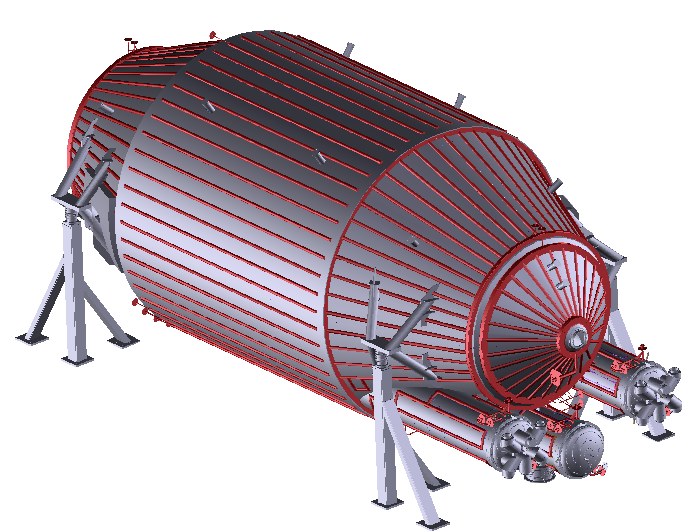
\includegraphics[width = \textwidth]{graphics/katrinExperiment/mainSpectrometer.jpg}
      	\end{minipage}
      	\begin{minipage}{0.29\textwidth}
      		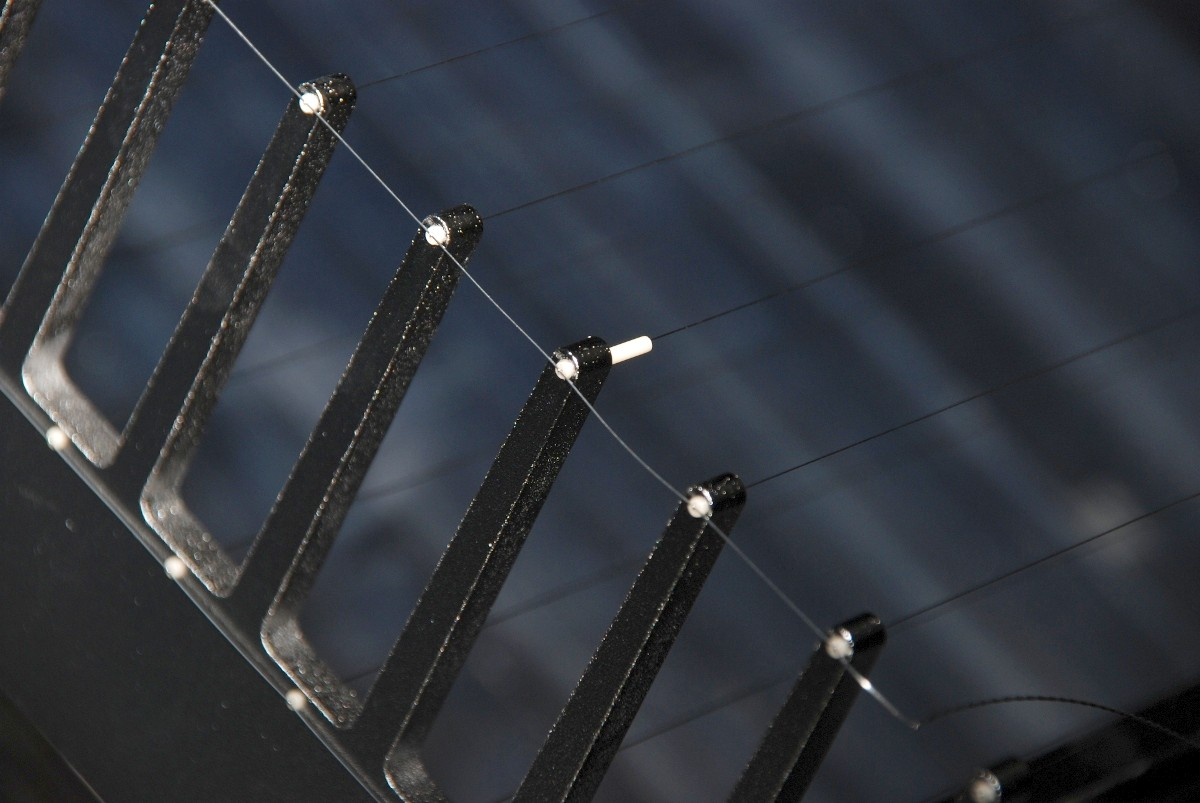
\includegraphics[angle = 90, width = \textwidth]{graphics/katrinExperiment/wireElectrodes.png}
      	\end{minipage}
      	\caption[Main Spectrometer and Wire Electrodes]{Left: the main spectrometer of the KATRIN experiment \cite{mainSpecStatus}. It is divided into a central part with cylindric shape to which the flat cones, and furthermore the steep cones, are attached. Also visible in this image are the 3 large pump ports on the lower right and the three-legged holding structures. On the right an image of the comb structure of the inner electrodes with both layers of wires is visible. The white structures on both top and bottom of the combs are required to insulate the wires from the combs, which are held on different potentials \cite{collabWireElectrodes}.}
      	\label{fig:mainSpec}
      \end{figure}
		
      \subsection{Monitor spectrometer}
      \label{ch:TheKATRINexperiment:sec:experimentalSetup:subsec:monSpec}
      
      The third MAC-E filter at KATRIN is the slightly modified Mainz spectrometer. It has been transported to Karlsruhe to work as a high voltage monitoring device. Here, electrons from $^{83m}$Kr decays are detected and analyzed. The fact that the energy from these decays does not change over time (neglecting changes in the source material) can be used to detect shifts in the voltage of the MAC-E filter. For that purpose, the monitor spectrometer constantly measures transmission functions of this particular L-32 line.
      The monitor spectrometer additionally features two scintillation modules for muon detection that were used for a first inspection of muon induced background.

     
      \subsection{Focal Plane Detector System}
      \label{ch:The KATRIN experiment:sec:Experimental setup:subsec:FPD system}
      The detector is located at the very north of the experiment. It consists of a silicon wafer whose back-side is divided into 148 pixels, as shown in figure \ref{fig:katrinExperiment:detectorWafer}, attached to the readout electronics by pin diode connectors. The pattern is dartboard-like where multiple pixels with the same distance to the center form rings. Every pixel has the same surface area, making rates more easily comparable - given that the magnetic flux through the wafer is sufficiently homogeneous.
      The detector system is roughly divided into two chambers: one connected to the ultra high vacuum of the main spectrometer and one with a lower grade vacuum on the detector's readout side.
      
      
      \begin{figure}
      \centering
	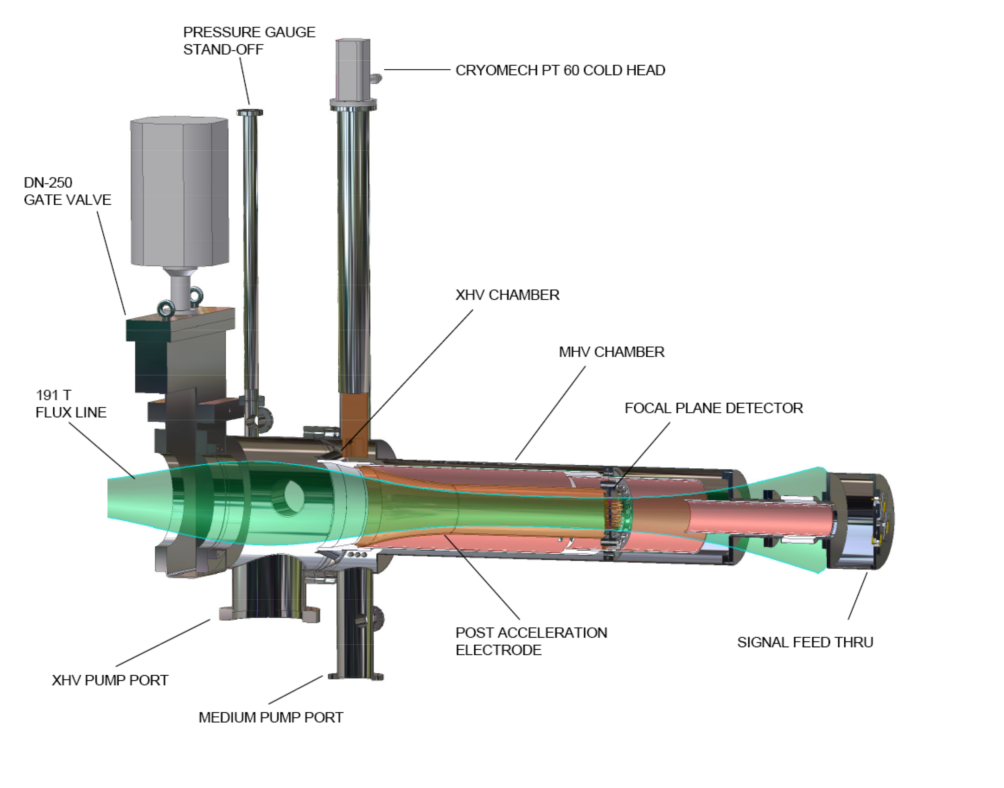
\includegraphics[width = 0.8 \textwidth]{graphics/katrinExperiment/detectorHousing.pdf}
	\caption[Focal Plane Detector system]{The focal plane detector system including the flux tube (green). The different grade vacuum sections can be identified: extremely high vacuum (XHV) and medium high vacuum (MHV). The post acceleration electrode is visible to the left of the bronze colored actual detector and its signal feed trough on the very right. Multiple flanges and connectors are shown. Not included in this picture are the calibration source holders \cite{FPD}.}
	\label{fig:katrinExperiment:detectorHousing}
      \end{figure}
      
      \begin{figure}
      \centering
      	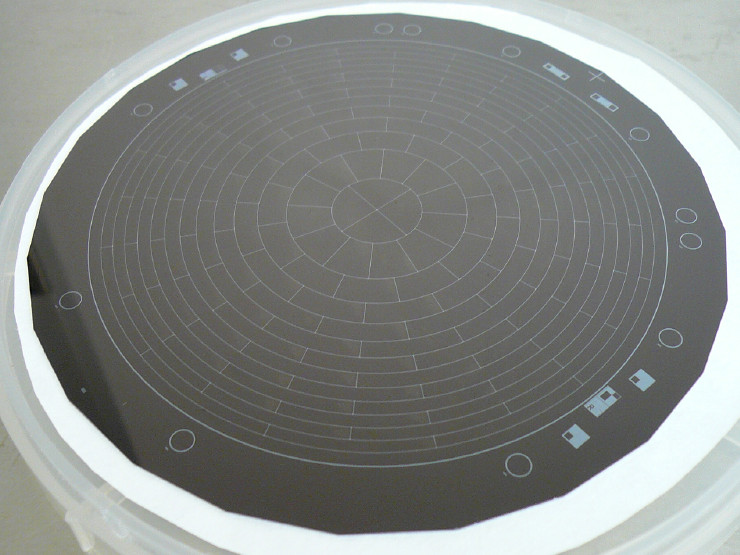
\includegraphics[width = 0.7 \textwidth]{graphics/katrinExperiment/detectorWafer.jpg}
	  \caption[Detector wafer]{The detector wafer as installed in the FPD system. Note the ``dartboard pattern'' with the four pixel bullseye in the center. This is the detectors back side to which the electronics are attached. The front is plaid making for high detection efficiencies.}
	  \label{fig:katrinExperiment:detectorWafer}
      \end{figure}
      
      
      For background reduction, the detector system features both a passive shielding and an active veto system read out by the same data crate as the detector itself. It allows to discriminate against externally induced detector events. Due to the high magnetic fields from the detector- and pinch magnet, semiconductor readout electronics had to be used instead of conventional photomultiplier tubes.
      As it may be necessary to investigate electrons with energies below the detector threshold, especially for background investigations, a post acceleration electrode has been installed - also visible in \ref{fig:katrinExperiment:detectorHousing}- that can add to the electrons' energies through an electric field of known strength.
      
      \subsection{Solenoids, LFCS and EMCS system}
      \label{ch:The KATRIN experiment:sec:Experimental setup:subsec:Solenoids, LFCS and EMCS system}
      
      To achieve magnetic guidance as explained in chapter \ref{ch:The KATRIN experiment:sec:Measurement Principle}, a sophisticated system of superconducting solenoids, the low field correction system LFCS and the earth magnetic field compensation system EMCS have been installed \cite{airCoilSystem}. These make sure that the path of flight is kept away from the wall and can be considered adiabatic, that penning traps are avoided as far as possible, that the earth magnetic field is compensated for and, most importantly, that the field drop towards the analyzing plane is of the order of \SI{e-4}{} such that the desired spectrometer resolution is achieved.
      

      \subsection{Background sources}
      \label{ch:The KATRIN experiment:sec:Experimental setup:subsec:BackgroundSources}
      The KATRIN experiment has a stringent background requirement of less than $10^{-2}$ counts per second (cps).
      Different sources contribute to the background of electrons arriving at the detector. Stored electrons are expected to be the largest source of detector background \cite{storedElectrons}. Penning traps cause electrons with energies in a certain range to be caught in a potential cup. Discharges of those traps due to scattering processes with either residual gas or due to excessive filling of the trap can cause high-rate events at the detector. Such discharges were observed to produce rates on the order of 100 kcps, which can even harm the detector. Stored electrons can be created by external sources or originate from within the spectrometer. One large background source is radon, a noble gas enabling it to move freely inside the vessel. Radon alpha decays produce high energy shake-off-, conversion- and Auger electrons which cool down via ionization of residual gas molecules. The thereby produced secondary electrons can be guided to the detector from inside the flux tube \cite{radonGoerhard, radonWandkowsky}.
      Another large background source that was already discussed above are cosmic rays interacting with the vessel hull thereby producing electrons. This background is reduced mainly by two factors, the symmetry of the magnetic field and the wire electrodes shielding the flux tube up to a certain threshold energy.
      If the fields, both electric and magnetic, were perfectly axially symmetric, only particles generated within the flux tube would be guided towards the detector. But through inhomogeneities and alignment errors, electrons may enter the flux tube through $E\times B$ drifts even if generated externally, e.g at the spectrometer wall. To suppress this background component, the wire electrodes, were installed. They shield the flux tube against electrons with energies up to $E_e = eU_{wire}$ depending on the wire electrodes voltage $U_{wire}$. 
      \begin{figure}
		\centering
		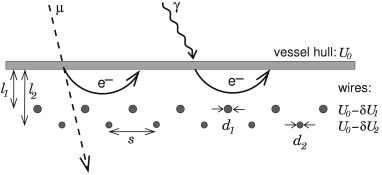
\includegraphics[width = 0.6\textwidth]{graphics/katrinExperiment/wireElectrodes.jpg}
		\caption[Wire Electrodes]{A graph of the wire electrodes installed inside the main spectrometer. Both layers of electrodes with different distances to the spectrometer wall are visible, the inner being smaller in diameter than the outer one. High energy photons can induce electrons, though the main component is generated by cosmic muons \cite{wireElectrodeSystem}.}
	  \end{figure}